\section{Introduction}

%\the\abovecaptionskip

% Urban modeling has made tremendous progress in the last decades by building on the availability of large-scale raw data (e.g., aerial images, Lidar scans, etc.) and advances in supervised machine learning algorithms. As a result, abstracted \textit{mass models} over large neighborhoods can automatically be created by analyzing aerial images and/or Lidar scans~\cite{Kelly:SIGA:2017}. In addition to being light weight, such models are often semantically structured, geographically tagged, and provide plausible abstractions of urban facades. 

We propose a framework to add geometric and texture details to coarse building models, commonly referred to as  {\em mass models}. There are multiple sources of such coarse models: they can be generated from procedural models, reconstructed from aerial images and \mbox{LIDAR} data, or created manually by urban planners, artists and architects. %designing  hypothetical cityscapes. % proposed or fictional new development.

% Urban modeling has made tremendous progress in the last decades by building on the availability of large-scale raw data (e.g., aerial images, Lidar scans, etc.) and advances in supervised machine learning algorithms. As a result, abstracted \textit{mass models} over large neighborhoods can automatically be created by analyzing aerial images and/or Lidar scans~\cite{Kelly:SIGA:2017}. In addition to being light weight, such models are often semantically structured, geographically tagged, and provide plausible abstractions of urban facades. 



% \paul{I think we should not pitch it too much as a reconstruction paper, we should make it clear that mass models can come from various sources (including manual and procedural generation) and need not come from reconstruction. The argument in the next paragraph alone may otherwise not be very convincing, since attaching rectified images can give results that are nicer than ours. Since we will probably detect the detail labels from the final images, the details would be just as good (or maybe better) than ours. The downside is that this is only possible if we want to reconstruct a real building.}


By themselves, these mass models lack geometric and texture details. They therefore look unrealistic when directly displayed.
For many applications, decorating these models by adding details that are automatically generated would be desirable. However, naive attempts to decorate mass models lead to unconvincing results. Examples include assigning uniform colors to different building fronts, `attaching' rectified street-view images (when available) to the mass model faces, or synthesizing facade textures using current generative adversarial networks (see Figure~\ref{fig:intro_naive}). A viable alternative is to use  rule-based procedural models, for both geometric and texture details. However, such an approach requires time and expertise. 
%
Instead, we build on the recent success of machine learning using generative adversarial networks (GANs) to simplify the modeling process and to learn facade details directly from real-world data. We focus on two issues 
%There are two issues with current work that we would like to improve upon
to make GANs suitable for our application.
First, current GANs are concerned only with the generation of textures, but we also require
semantic and geometric details
for our urban modeling applications.
Second, current GANs provide little \textit{style control}. We would like to improve control over the style of facade details. For example, a user may wish to decorate a mass model in the style of a given example facade, or to specify how similar facades should be within an urban neighborhood. %automatically decorated block of mass models.
% \paul{possible additional challenge with directly using GANs: facades have a complex structure that is hard to generate end-to-end. (Current end-to-end results from blank facade to an image often look worse than ours since they don't have window layout ground truth as guidance.)}

%making the synthesis of details with realistic variation across different styles difficult.
%\twak{Manual texturing is time-consuming, even for skilled artists: UV coordinates must be defined, as well as specular, [normal], and texture bitmaps. Manual texturing, and procedural modeling are highly subjective, ignoring the large datasets available today.} Such an assisted workflow does not scale to detail large-scale models and across different styles. 
% (e.g. Sylvains paper\cite{xx})

\begin{figure}[t!]
    \centering
    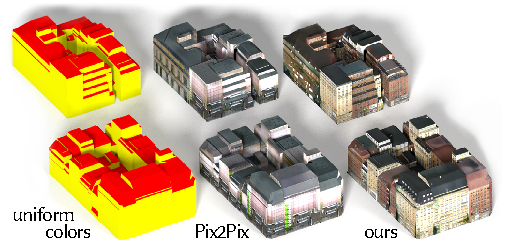
\includegraphics[width=\columnwidth]{images/intro_naive.pdf}
    \vspace{-10pt}
    \caption{Naive options to texture a mass model give unconvincing results. Pix2Pix shows heavy mode collapse, discussed in Section~\ref{sec:qualitative_comparisons}.}
    \label{fig:intro_naive}
    \vspace{-5pt}
\end{figure}


\begin{figure*}[t!]
    \centering
    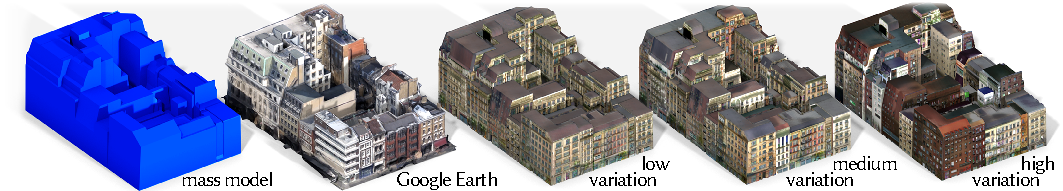
\includegraphics[width=\textwidth]{images/style_variation_teaser.pdf}
    \caption{In contrast to photogrammetric reconstruction (second column), our method can be used to synthesize new facade layouts and textures. Style and variation can be controlled by the user; in columns 3 to 5, we show details generated by \systemName with low to high style variation.}
    \label{fig:photogrammetric}
\end{figure*}

Here, we consider the problem of automatically and realistically {\em detailing} mass models using user-supplied building images for style-guidance, with the option to adjust style variety. By details, we refer to both geometric and texture, details. Geometric details include balconies, window frames, roof types, chimneys, etc., while texture details refer to realistic facade appearances that are consistent with (latent) semantic elements such as windows, sills, etc. Further, we require the added details to be stylistically consistent and guided by user-provided input image(s). We do {\em not} expect the input images to be semantically-annotated or to correspond to the target mass models. 
%
The output of our algorithm (see Figure~\ref{fig:teaser}) is a mixture of 2.5D geometry with textures and realistic variations.

%\twak{ instead of being procedurally  instantiated. - balconies are procedural... }


Technically, we perform detailing in stages via a cascade of GANs. We engineer the individual GANs to generate particular styles that are encoded as latent vectors. As a result, we can synchronize the different GAN outputs by selecting style vectors from appropriate distributions. We demonstrate how to perform such style-guided synthesis for both geometric and texture details. By allowing style vectors to be guided by input images, we allow users to perform, at interactive rates, drag-and-drop stylization by simply providing  different target images  (see supplementary video).  
Our system, called \systemName, ensures that the resultant detailed models are realistic and are stylistically consistent both within individual buildings and between buildings in a neighborhood. 
 


%para 5: demonstrate on various datasets .. 
We test our system by detailing a variety of mass models over large-scale city neighborhoods. We then compare the quality of the detailed models against baseline alternatives using a perceptual study. In summary, our main contributions are: 
(i)~introducing the problem of realistically {\em detailing} mass models with semantically consistent geometric and texture details; 
(ii)~presenting \systemName as an interactive system that utilizes latent style vectors via a cascade of synchronized GANs guided by examplar style images; and 
(iii)~demonstrating the system on several large-scale examples and qualitatively evaluating the generated output.
%
\changed{Source code and pre-trained networks are available at \emph{\url{http://geometry.cs.ucl.ac.uk/projects/2018/frankengan/}}.}





\if0
Main motivation:
\begin{itemize}
    \item multiple facade's labels to textured facades of the same style
    \item single labels to many textures facades of diverse styles
\end{itemize}

We should have a single network that is able to achieve both of these goals. By conditioning the latent space on both input-input and output-output distances, we are able to achieve the above results.

Other applications:

\begin{itemize}
    \item facade completion (few windows to many windows)
    \item texture suggestions (given the wooden door, suggests some different styles of wooden windows)
    \item consistent super-resolution. Zoom into two different locations on a single high resolution facade. Observe the same small-scale features.
\end{itemize}

Potential technical contributions:
\begin{itemize}
    \item the idea of using any distance measure for the latent space has an attractive simplicity over prior disentanglement formulations 
    \item improving standard pix2pix (unet + gan) with improved loss function, and ...?
    \item multiple latent spaces (e.g. one for lat/long distance and another for VGG 19 layer 3 activation distance). Does this count as disentanglement? Is it just as fast?
    \item show that the concept works on other network architectures (cyclegan, pix2pixHD)
    \item generation results are fast / real-time
\end{itemize}
\fi


% \begin{figure*}[t]
%     \centering
%     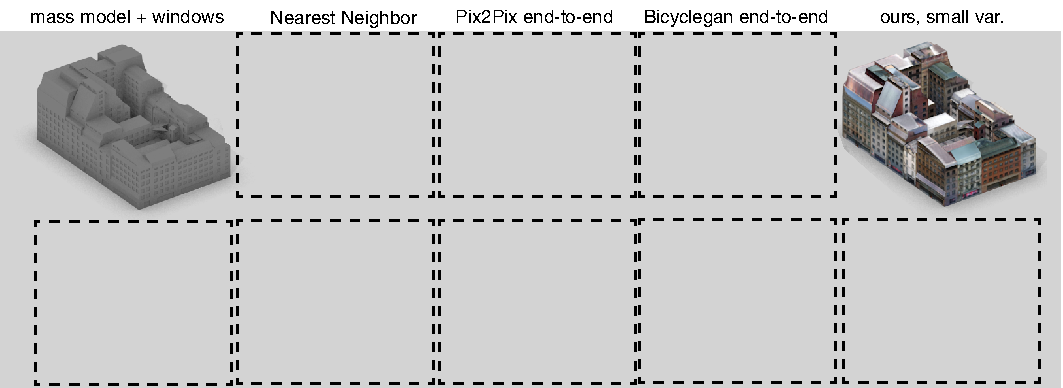
\includegraphics[width=\textwidth]{images/comparison_endtoend.pdf}
%     \caption{Splitting detail generation into multiple steps gives higher-quality than single-step approaches that are trained end-to-end. Using multiple steps provides more guidance during training and allows for a larger total network capacity for a given amount of GPU memory, since the networks for each step do not need to be loaded at the same time.}
%     \label{fig:intro_comparison_endtoend}
% \end{figure*}